\chapter{Implementation of the Trading Systems}
This section provides a comprehensive overview of the two trading system implementations. The first one focuses on the backtesting system, which involves simulating and evaluating strategies in a controlled environment. In this system, historical market data is utilized to test and analyze the performance of various strategies. The second implementation is the live system, designed to execute trades on the Ethereum blockchain using smart contracts. This system operates in real-time and interacts with the live market, allowing for actual trades to be executed based on predefined strategies. Together, these two implementations provide a comprehensive framework for testing, evaluating, and deploying trading strategies, both in simulated environments and on the live blockchain.

\section{Buying and Selling}
The process of buying and selling in traditional markets is relatively straightforward as brokers and exchanges play a crucial role in executing orders on behalf of individuals. However, when it comes to trading cryptocurrencies, the responsibility falls directly on the trader, such as myself. Therefore, it becomes essential to clearly define what buying and selling entail in the context of cryptocurrency trading.

\subsection{Buying}
Prices on Uniswap are represented as ratios for example 1 USDC = $P$ WETH. With this understanding, let's delve into the process of buying one unit of USDC/WETH on Uniswap:
\begin{itemize}
    \item Opening a Buy position:\begin{itemize}
        \item Starts with $P_{0}$ WETH
        \item Swaps the WETH for USDC, hence ends with 1 USDC
    \end{itemize}
    \item Closing a Buy position:\begin{itemize}
        \item Starts with 1 USDC
        \item Swaps the USDC for WETH, hence ends with $P_1$ WETH
    \end{itemize}
\end{itemize}
\noindent Consequently, if the price of USDC/WETH increases from the moment the buy position is opened to the time it is closed, the trader realizes a profit. On the other hand, if the price declines during this period, the trader incurs a loss.

\subsection{Selling}
Selling an asset is a more complex process compared to buying because it involves trading an asset that the trader doesn't initially possess. In traditional markets, this is facilitated by the trader borrowing the desired asset from a broker or another party. When the trader decides to close the position, they repurchase the same amount of the borrowed asset and return it to the lender, hoping that its value has declined. This borrowing and returning process is typically managed automatically by brokers and exchanges. However, in decentralized exchanges (DEXes), such mechanisms are not in place.
\\[5mm]
To simplify this process, I have opted to utilize Aave as a lending platform to borrow any required assets. It is worth noting that Aave supports only a limited range of tokens available for borrowing, namely DAI, EURS, USDC, USDT, AAVE, LINK, WBTC, and WETH. Therefore, shorting would be feasible only if I focus on liquidity pools that involve these cryptocurrencies. By leveraging Aave as a lending platform, I can access the necessary assets for shorting. The process of selling is as follows:
\begin{itemize}
    \item Opening a Sell position:\begin{itemize}
        \item Borrow 1 USDC
        \item Swaps the USDC for WETH, hence ends with $P_0$ WETH
    \end{itemize}
    \item Closing a Sell position:\begin{itemize}
        \item Starts with $P_0$ WETH
        \item Swaps the WETH for USDC, hence ends with $\frac{P_0}{P_1}$ USDC
        \item Return the borrowed USDC, leaving $\frac{P_0}{P_1} - 1$ USDC
    \end{itemize}
\end{itemize}
Consequently, if the price of USDC/WETH decreases, i.e. $P_1 < P_0$ from the moment the sell position is opened to the time it is closed, the trader realizes a profit. On the other hand, if the price increases during this period, the trader incurs a loss.
\\[5mm]
Note that this is is merely an illustrative example and does not account for any potential fees that the trader might incur.

\section{Backtesting System}

To develop a resilient backtesting system, a dedicated class was constructed to streamline the process of testing trading strategies. Upon evaluating a particular strategy the \texttt{backtest} function requires \texttt{cointegrated\_pair}, a tuple of the names of the liquidity pools that the strategy is to be evaluated on, \texttt{strategy}, the strategy, and finally, the \texttt{initial\_investment} in ETH. The first argument is required and used to retrieve the relevant historical prices. The second parameter is self-explanatory, the strategy to test. Finally, the inclusion of the initial investment amount as an input parameter enables users to simulate the performance of their strategies with a specific starting capital, it also helps analyze how the various transaction costs affect the ability to trade if any trades do result in a loss. The \texttt{backtest} function iterates through historical data calling the strategy's \texttt{generate\_signal} and executing the trade orders it receives at each timestep. However, to do this historical data is required hence, the first step is to collect the historical data.

\subsection{Data Collection and Storage}
In order to simulate the market as accurately as possible the system should have access to reliable and accurate historical market data, including price, volume, and other relevant indicators. Therefore, I retrieve all of my data from the Uniswap and Aave protocols' subgraph using the Graph~\cite{noauthor_graph_nodate}. The Graph is a decentralized protocol for indexing and querying blockchain data hence making the data provided 100\% reliable as it indexes directly on the Ethereum blockchain. Subgraphs serve as GraphQL APIs designed to facilitate querying and extracting data from the blockchain. These APIs adhere to a specific schema outlined by the protocol, enabling seamless communication between the protocol and the underlying blockchain. Therefore, I employ the Uniswap V3, Aave V2, and Aave V3 subgraphs to obtain the data required for the backtesting system.
\\[5mm]
The database has the following tables:
\begin{figure}[!htb]
    \centering
    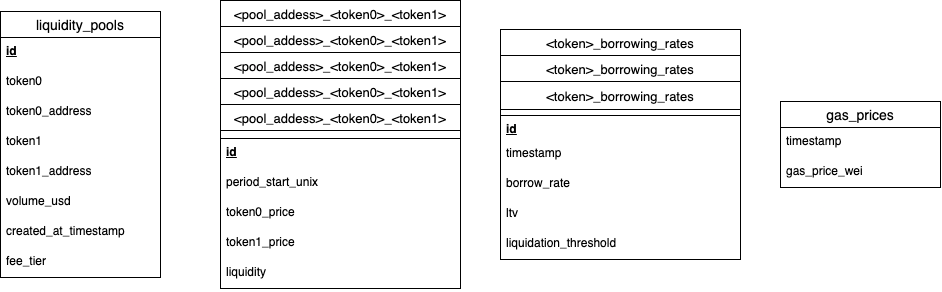
\includegraphics[width=0.8\textwidth]{project/Images/database_tables.png}
    \caption{Tables contained in the database \label{fig:database}}
\end{figure}
The \texttt{liquidity\_pools} contains data about the liquidity pools that exist on Uniswap V3. After obtaining all of the data it is found that it possesses 12,182 liquidity pools. However, a substantial portion of these pools exhibit minimal or negligible trading volume. As a result, a criterion is established to selectively include only those liquidity pools that involve tokens supported by Aave and possess a trading volume exceeding \$10,000,000 (or \$10 million). This filtering condition ensures that the collected and stored data holds significance and relevance for research purposes, as these pools would allow for short selling.
\\[5mm]
Once these pools have been identified, pricing data about each pool that meets this condition is collected again using the Uniswap V3 subgraph. The following shows the GraphQL query:
\vspace{5mm}
\begin{lstlisting}
query ($id: ID!, $prev_max_time: Int!) {
    pool(id: $id) {
        poolHourData(where: {periodStartUnix_gt: $prev_max_time}, orderBy: periodStartUnix, first: 1000) {
            id
            token0Price
            token1Price
            periodStartUnix
            liquidity
            feesUSD
        }
    }
}
\end{lstlisting}
\vspace{5mm}
This query returns an array of dictionaries containing the pre-specified pricing datapoints at a frequency of every hour. Due to the limitations imposed by the subgraph, the results are constrained to a maximum size of 1000 entries. To overcome this limitation and obtain the complete dataset, the query is executed iteratively. The previous maximum time, referred to as \texttt{prev\_max\_time}, is passed as an argument in subsequent queries to fetch the remaining data, i.e. \texttt{prev\_max\_time = hourlyData[-1]['periodStartUnix'] if len(hourlyData) > 0 else prev\_max\_time}. This data is stored in tables of the form \textit{<pool\_address>}\_\textit{<token0>}\_\textit{<token1>}.
\\[5mm]
In a similar manner, obtaining the interest rates for borrowing necessitates the utilization of two of Aave's subgraphs. This requirement arises due to Aave's migration to Version 3 in March 2022, resulting in a transitional period where both Uniswap V3 and Aave V2 were concurrently utilized. The schemas for the two are different, however for the data we require, the borrowing rate, loan-to-value and liquidity threshold, the schema is consistent and the same query can be used:
\vspace{5mm}
\begin{lstlisting}
query ($symbol: String!, $prev_max_time: Int!) {
    reserves(where: {symbol: $symbol}) {
        id
        symbol
        lifetimeBorrows
        baseLTVasCollateral
        reserveLiquidationThreshold
        borrowHistory(
            where: {timestamp_gt: $prev_max_time}, first: 1000, orderBy: timestamp, orderDirection: asc) {
            id
            timestamp
            borrowRate
        }
    }
}
\end{lstlisting}
\vspace{5mm}
During the table initialization process, requests are made to both the V2 and V3 GraphQL endpoints. However, when updating the table, only the V3 endpoint is utilized for sending requests. The data is stored in tables of the form \textit{<symbol>}\_borrowing\_rates, where \textit{<symbol>} are all of the tokens that are present in the liquidity pools that are of interest.
\\[5mm]
To collect the gas price history, the transaction history is queried at each hour since Uniswap migrated to V3. This is because querying in the same as the pricing data and borrowing rate history is too exhaustive as transactions occur every second. Therefore, it is more efficient to query at each hour with a window to retrieve the gas price at the closest hour as follows:
\vspace{5mm}
\begin{lstlisting}
query ($min_time: Int!, $max_time: Int!) {
    transactions(where: {timestamp_gt: $min_time, timestamp_lt: $max_time}, first:1000, orderBy: timestamp, orderDirection: asc) {
        id
        timestamp
        gasPrice
    }
}
\end{lstlisting}
\vspace{5mm}
The following pseudocode shows how to fetch the gas price at each hour:

\begin{algorithm}
    \caption{Retrieval of hourly gas prices where $min\_time$ \& $max\_time$ are arguments}\label{alg_gas_price_col}
    \begin{algorithmic}
        \State $rows\_set \leftarrow \{\}$
        \For{$timestamp$ from $min\_time$ to $max\_time + (60 \times 60), step\_size = (60 \times 60)$}
            \State $found\_result \leftarrow False$
            \State $window\_size\_in\_minutes \leftarrow 5$
            \While{$not\ found\_result$}
                \State $transaction\_data \leftarrow$ GraphQL Query with arguments: $\{``min\_time": timestamp - (60 * window\_size\_in\_minutes), ``max\_time": timestamp + (60 * window\_size\_in\_minutes)\}$
                \If{$transaction\_data != 0$}
                    \State $transaction\_data\_sorted = sorted(transaction\_data, key=lambda\ x:abs(timestamp - int(x['timestamp'])))$
                    \State $rows\_set.update({timestamp: (timestamp, transaction\_data\_sorted[0]['gasPrice'])})$
                    \State $found\_result \leftarrow True$
                \Else
                    \State $window\_size\_in\_minutes \leftarrow window\_size\_in\_minutes + 5$
                \EndIf
            \EndWhile
            \State insert $rows\_set[timestamp]$ into \texttt{gas\_prices} table
        \EndFor
    \end{algorithmic}
\end{algorithm}

\subsection{Types of Orders and Execution}
There are numerous order types that the backtesting supports due to measures to enusre a positive balance and avoid liquidation. The types of orders are; \texttt{BUY\ ETH}, \texttt{WITHDRAW}, \texttt{DEPOSIT}, \texttt{SWAP}, \texttt{OPEN\ BUY}, \texttt{CLOSE\ BUY}, \texttt{OPEN\ SELL}, \texttt{CLOSE\ SELL}. The precedures of each are outlined below.

\subsubsection{\texttt{BUY\ ETH}}
The \texttt{BUY\ ETH} order is used to swap a percentage of the accounts balance from WETH to ETH. The arguments is an float between 0 and 1. The logic of the execution, excluding gas fees, of the order is outlined below.
\vspace{5mm}
\begin{lstlisting}[language=Python]
amount_to_swap = self.account['WETH'] * order[1]
self.account['WETH'] = self.account['WETH'] - amount_to_swap
self.account['ETH'] = self.account['ETH'] + amount_to_swap
\end{lstlisting}

\subsubsection{\texttt{SWAP}}
The \texttt{SWAP} order is to execute a simple swap for either token0 or token1 of the liquidity pool. This order is only used as a precautionary order, if the balance of the WETH balance gets too low. It takes 2 arguments, the first indicating whether it is swapping for token0 or token1 and the second parameter is a list of swaps, tuples containing with pool and the quantity, that would like to be swapped. As can be seen in the code excerpt below, the amount received in the account is multiplied by \texttt{(1 - swap\_fees[swap\_token])}, this is because Uniswap charges a percentage of the swap specified by \texttt{swap\_fees[swap\_token]}.
\vspace{5mm}
\begin{lstlisting}[language=Python]
if is_for_token0:
    for swap_for_token0 in swaps:
        swap_token, swap_volume = swap_for_token0
        self.account['WETH'] = self.account['WETH'] - (swap_volume * prices[f'P{swap_token[1]}'])
        self.account[swap_token] = self.account[swap_token] + (swap_volume * (1 - swap_fees[swap_token]))
else:
    for swap_for_token1 in swaps:
        swap_token, swap_volume = swap_for_token1
        self.account[swap_token] = self.account[swap_token] - (swap_volume / prices[f'P{swap_token[1]}'])
        self.account['WETH'] = self.account['WETH'] + (swap_volume * (1 - swap_fees[swap_token]))
\end{lstlisting}

\subsubsection{\texttt{OPEN\ BUY}}
Similar to the \texttt{SWAP} order, \texttt{OPEN\ BUY} opens a buy position. As mentioned above opening a buy order is simply swapping token1 for token0. The parameters of buying are the target token and the volume. 
\vspace{5mm}
\begin{lstlisting}[language=Python]
self.account['WETH'] = self.account['WETH'] - (volume * buy_price)
self.account[token] = self.account[token] + (volume * (1 - swap_fees[token]))
\end{lstlisting}

\subsubsection{\texttt{CLOSE\ BUY}}
Closing a buy position is similar to opening a buy position, however, the swap is in the other direction, i.e. from token to WETH. The only argument is the id of the buy order. To account for Uniswap's fees, the volume that was received, after the initial swap, is calculated then this volume is swapped back to WETH.
\vspace{5mm}
\begin{lstlisting}[language=Python]
buy_token, bought_price, buy_volume, buy_timestamp = self.open_positions['BUY'][buy_id]
volume_bought = buy_volume * (1 - swap_fees[buy_token])
self.account[buy_token] = self.account[buy_token] - volume_bought
self.account['WETH'] = self.account['WETH'] + (prices[f'P{buy_token[1]}'] * (volume_bought * (1 - swap_fees[buy_token])))
\end{lstlisting}

\subsubsection{\texttt{OPEN\ SELL}}
Opening a sell position involves borrowing a token and then swapping the token. The parameters of selling are the target token and the volume. It also consists of depositing the required amount to borrow the volume ordered, calculated by the value to loan ratio.
\vspace{5mm}
\begin{lstlisting}[language=Python]
# Borrow token and Deposit collateral
amount_to_move_to_collateral_WETH = ((volume * sell_price) / ltv_eth)
self.account[token] = self.account[token] + volume
self.account['WETH'] = self.account['WETH'] - amount_to_move_to_collateral_WETH
self.account['collateral_WETH'] = self.account['collateral_WETH'] + amount_to_move_to_collateral_WETH

# Swap borrowed tokens to WETH
self.account[token] = self.account[token] - volume
self.account['WETH'] = self.account['WETH'] + (volume * (1 - swap_fees[token]) * sell_price)
\end{lstlisting}

\subsubsection{\texttt{CLOSE\ SELL}}
Closing a sell position is more complicated that as in requires to swap back from the token to WETH, repay the loan with interest and finally return collateral. Swapping back to the required amount of tokens is the first step. For this the variable Annual Yield Rates between the timestamp of the opening of the position and closing positon is used to calculate the amount of interest required to be paid as this is cumulated every second. Once the volume of tokens required to be returned is calculated, the equivelent amount of WETH plus accounting for Uniswap fees is swapped to obtain these tokens. Finally, the tokens are repayed and the collateral is returned.
\vspace{5mm}
\begin{lstlisting}[language=Python]
sell_token, sold_price, sell_volume, sell_timestamp = self.open_positions['SELL'][sell_id]

# Swap WETH back to Token
volume_required_to_return = sell_volume
previous_timestamp = sell_timestamp

for apy_idx in apy[sell_token].index:
    local_apy = apy[sell_token].loc[apy_idx]['borrow_rate']
    number_of_seconds = apy[sell_token].loc[apy_idx]['timestamp'] - previous_timestamp
    secondly_yield = (1 + local_apy)**(1 / (365*24*60*60))
    volume_required_to_return *= secondly_yield ** number_of_seconds
    previous_timestamp = apy[sell_token].loc[apy_idx]['timestamp']

self.account['WETH'] = self.account['WETH'] - (sold_price * volume_required_to_return / (1 - swap_fees[sell_token])) 
self.account[sell_token] = self.account[sell_token] + volume_required_to_return

# Return Borrowed Tokens and Collatoral
self.account[sell_token] = self.account[sell_token] - volume_required_to_return
self.account['WETH'] = self.account['WETH'] + self.account['collateral_WETH']
self.account['collateral_WETH'] = 0
\end{lstlisting}

\subsubsection{\texttt{WITHDRAW}}
The \texttt{WITHDRAW} order's function is to withdraw some collateral that is stored in Aave. It is not used in the strategies however is implemented in case of developing further strategies that may require this functionality. The only parameter is the amount that would like to be withdrawn.
\vspace{5mm}
\begin{lstlisting}[language=Python]
self.account['WETH'] = self.account['WETH'] + withdraw_amount
self.account['collateral_WETH'] = self.account['collateral_WETH'] - withdraw_amount
\end{lstlisting}

\subsubsection{\texttt{DEPOSIT}}
The \texttt{DEPOSIT} order's function is to deposit some additional collateral that is stored in Aave. This order is used when the collateral value not properly covering the loan value, hence avoiding liquidation. The only parameter is the amount that would like to be depositted. 
\vspace{5mm}
\begin{lstlisting}[language=Python]
self.account['WETH'] = self.account['WETH'] - deposit_amount
self.account['collateral_WETH'] = self.account['collateral_WETH'] + deposit_amount
\end{lstlisting}

\subsection{Gas Fees - TODO}

\subsection{Validating Balance Health}
To maintain the integrity and effectiveness of the trading strategy, it is crucial to incorporate various checks and safeguards after each trade and at each timestep. One key aspect involves monitoring the balance of each token to ensure that it remains positive. After every order execution, the balances of the tokens involved are checked, and if any of them fall below zero, an exception is triggered.
\vspace{5mm}
\begin{lstlisting}[language=Python]
if self.account['T1'] < negative_threshold:
    raise Exception('Account balace goes below 0 - T1')

if self.account['T2'] < negative_threshold:
    raise Exception('Account balace goes below 0 - T2')

if self.account['WETH'] < negative_threshold:
    raise Exception('Account balace goes below 0 - WETH')

if self.account['ETH'] < negative_threshold:
    raise Exception('Account balace goes below 0 - ETH')
\end{lstlisting}
\vspace{5mm}    
Furthermore, to simulate the potential liquidation of a sell position's loan, the loan-to-value ratio is calculated. This ratio serves as an indicator of the position's health and risk level. If the loan-to-value ratio breaches the predefined liquidation threshold, indicating that the position is approaching an unsustainable state, an exception is thrown.
\vspace{5mm}
\begin{lstlisting}[language=Python]
sell_token, sold_price, sell_volume, _ = sell_trade
current_token_price = prices[f'P{sell_token[1]}']
curr_value_of_loan_pct = (sell_volume * current_token_price) / self.account['collateral_WETH']
if round(curr_value_of_loan_pct, 4) > liquidation_threshold:
    raise Exception(f'Short position liquidated')
\end{lstlisting}

\section{Live Trading - TODO}
